% !TeX program = pdfLaTeX
\documentclass[12pt]{article}
\usepackage{amsmath}
\usepackage{graphicx,psfrag,epsf}
\usepackage{enumerate}
\usepackage{natbib}
\usepackage{textcomp}
\usepackage[hyphens]{url} % not crucial - just used below for the URL
\usepackage{hyperref}
\providecommand{\tightlist}{%
  \setlength{\itemsep}{0pt}\setlength{\parskip}{0pt}}

%\pdfminorversion=4
% NOTE: To produce blinded version, replace "0" with "1" below.
\newcommand{\blind}{0}

% DON'T change margins - should be 1 inch all around.
\addtolength{\oddsidemargin}{-.5in}%
\addtolength{\evensidemargin}{-.5in}%
\addtolength{\textwidth}{1in}%
\addtolength{\textheight}{1.3in}%
\addtolength{\topmargin}{-.8in}%

%% load any required packages here



% Pandoc citation processing

\usepackage[dvipsnames]{xcolor} % colors
\newcommand{\ear}[1]{{\textcolor{blue}{#1}}}
\newcommand{\svp}[1]{{\textcolor{RedOrange}{#1}}}
\newcommand{\rh}[1]{{\textcolor{Green}{#1}}}
\usepackage[capitalise]{cleveref}
\newcommand\pcref[1]{(\cref{#1})}
\usepackage{algorithm,algpseudocode,booktabs}

\begin{document}


\def\spacingset#1{\renewcommand{\baselinestretch}%
{#1}\small\normalsize} \spacingset{1}


%%%%%%%%%%%%%%%%%%%%%%%%%%%%%%%%%%%%%%%%%%%%%%%%%%%%%%%%%%%%%%%%%%%%%%%%%%%%%%

\if0\blind
{
  \title{\bf Eye Fitting Straight Lines in the Modern Era}

  \author{
        Emily A. Robinson 1 \\
    Department of Statistics, University of Nebraska - Lincoln\\
     and \\     Susan VanderPlas 2 \\
    Department of Statistics, University of Nebraska - Lincoln\\
     and \\     Reka Howard 3 \\
    Department of Statistics, University of Nebraska - Lincoln\\
      }
  \maketitle
} \fi

\if1\blind
{
  \bigskip
  \bigskip
  \bigskip
  \begin{center}
    {\LARGE\bf Eye Fitting Straight Lines in the Modern Era}
  \end{center}
  \medskip
} \fi

\bigskip
\begin{abstract}
Fitting lines by eye through a set of points has been explored since the
20th century. Common methods of fitting trends by eye involve
maneuvering a string, black thread, or ruler until the fit is suitable,
then drawing the line through the set of points. In 2015, the New York
Times introduced an interactive feature, called `You Draw It'. Readers
are asked to input their own assumptions about various metrics and
compare how these assumptions relate to reality. The New York Times team
utilizes Data Driven Documents (D3) that allows readers to predict these
metrics by drawing a line on their computer screen with their computer
mouse. In my research, I established `You Draw It' as a method for
graphical testing by adapting the New York Times feature. I recruited
participants via crowdsourcing websites and replicated the study found
in Eye Fitting Straight Lines (Mosteller et al., 1981). Participants
were directed to an RShiny application link and shown points following a
linear trend and asked to draw a line through the data points using
their computer mouse; task plots were generated using the r2d3 package
in R statistical software. Results from my study were consistent with
those found in the previous study; when shown points following a linear
trend, participants tended to fit the slope of the first principal
component over the slope of the least-squares regression line. This
trend was most prominent when shown data simulated with larger
variances. The reproducibility of these results serves as evidence of
the reliability of the you draw it method. Future work is necessary to
implement the `You Draw It' tool as a method of testing graphics. {[}200
word limit{]}
\end{abstract}

\noindent%
{\it Keywords:} Graphics, Regression, Graph
Perception, Scatterplot, Cognitive Bias
\vfill

\newpage
\spacingset{1.45} % DON'T change the spacing!

\hypertarget{introduction}{%
\section{Introduction}\label{introduction}}

\begin{itemize}
\tightlist
\item
  What are graphs? Why do we care?
\end{itemize}

\hypertarget{graph-perception}{%
\subsection{Graph Perception}\label{graph-perception}}

\begin{itemize}
\tightlist
\item
  \citet{cleveland1984graphical}
\item
  \citet{cleveland1985graphical}
\end{itemize}

\hypertarget{testing-statistical-graphics}{%
\subsection{Testing Statistical
Graphics}\label{testing-statistical-graphics}}

Graphical tests are useful for studying the perception of statistical
graphs. Studies might ask participants to identify differences in
graphs, read information off of a chart accurately, use data to make
correct real-world decisions, or predict the next few observations. All
of these types of tests require different levels of use and manipulation
of the information being presented in the chart. Early researchers
studied graphs from a psychological perspective
\citep{spence1990visual, lewandowsky1989perception}. These studies
generally tested participants ability to detect a stimulus or a
difference between two stimuli. Here we focus on the how graphical
testing has developed in statistics.

A major development in statistical graphics research is Wilkinson's
Grammar of Graphics \citep{wilkinson2013grammar}. The grammar of
graphics serves as the fundamental framework for data visualization with
the notion that graphics are built from the ground up by specifying
exactly how to create a particular graph from a given data set. Visual
representations are constructed through the use of ``tidy data'' which
is characterized as a data set in which each variable is in its own
column, each observation is in its own row, and each value is in its own
cell \citep{wickham2016r}. Graphics are viewed as a mapping from
variables in a data set (or statistics computed from the data) to visual
attributes such as the axes, colors, shapes, or facets on the canvas in
which the chart is displayed. Software, such as Hadley Wickham's ggplot2
\citep{wickham2011ggplot2}, aims to implement the framework of creating
charts and graphics as the grammar of graphics recommends.

One useful tool for testing statistical graphics is the concept of a
lineup. \citet{buja2009statistical} introduced the lineup protocol in
which data plots are depicted and interpreted as statistics. Supported
by the grammar of graphics, a data plot can be characterized as a
statistic, defined as, ``a functional mapping of a variable or set of
variables'' \citep{vanderplas2020testing}. This allows the data plot to
be tested similar to other statistics, by comparing the actual data plot
to a set of plots with the absence of any data structure we can test the
likelihood of any perceived structure being significant. The
construction of data plots as statistics allow for easy experimentation,
granting researchers the ability to compare the effectiveness of and
understand the perception of different types of charts
\citep{vanderplas2017clusters, vanderplas2015spatial, hofmann2012graphical}.
The lineup protocol is one such example of the development of tools
designed for statistical graphical testing. The advancement of graphing
software provides the tools necessary to develop new methods of testing
graphics.

\hypertarget{fitting-trends-by-eye}{%
\subsection{Fitting Trends by Eye}\label{fitting-trends-by-eye}}

Initial studies in the 20th century explored the use of fitting lines by
eye through a set of points
\citep{finney1951subjective, mosteller1981eye}. Common methods of
fitting trends by eye involved maneuvering a string, black thread, or
ruler until the fit is suitable, then drawing the line through the set
of points. Recently, \citet{ciccione2021can} conducted a comprehensive
set of studies investigating human ability to detect trends in graphical
representations from a psychophysical approach.

In \citet{finney1951subjective}, it was of interest to determine the
effect of stopping iterative maximum likelihood calculations after one
iteration. Many techniques in statistical analysis are performed with
the aid of iterative calculations such as Newton's method or Fisher's
scoring. The author was interested in whether one iteration of
calculations was sufficient in the estimation of parameters connected
with dose-response relationships. One measure of interest is the
relative potency between a test preparation of doses and standard
preparation of does; relative potency is calculated as the ratio of two
equally effective doses between the two preparation methods. In this
study, twenty-one scientists were recruited via postal mail and asked to
``rule two lines'' in order to judge by eye the positions for a pair of
parallel probit regression lines in a biological assay. The author then
computed one iterative calculation of the relative potency based on
starting values as indicated by the pair of lines provided by each
participant and compared these relative potency estimates to that which
was estimated by the full probit technique (reaching convergence through
multiple iterations). Results indicated that one cycle of iterations for
calculating the relative potency was sufficient based on the starting
values provided by eye from the participants.

\citet{mosteller1981eye}, sought to understand the properties of least
squares and other computed lines by establishing one systematic method
of fitting lines by eye. Participants were asked to fit lines by eye to
four scatter-plots using an 8.5 x 11 inch transparency with a straight
line etched completely across the middle. A latin square design with
packets of the set of points stapled together in four different
sequences was used to determine if there is an effect of order of
presentation. It was found that order of presentation had no effect and
that participants tended to fit the slope of the principal axis (error
minimized orthogonally, both horizontal and vertical, to the regression
line) over the slope of the least squares regression line (error
minimized vertically to the regression line). These results support
previous research on ``ensemble perception'' indicating the visual
system can compute averages of various features in parallel across the
items in a set
\citep{chong2003representation, chong2005statistical, van2011rapid}.

In \citet{ciccione2021can}, participants were asked to judge trends,
estimate slopes, and conduct extrapolation. To estimate slopes,
participants were asked to report the slope of the best-fitting
regression line using a trackpad to adjust the tilt of a line on screen.
Results indicated the slopes participants reported were always in excess
of the ideal slopes, both in the positive and in the negative direction,
and those biases increase with noise and with number of points. This
supports the results found in \citet{mosteller1981eye} and suggest that
participants might use Deming regression when fitting a line to a noisy
scatterplot.

In 2015, the New York Times introduced an interactive feature, called
You Draw It
\citep{aisch_cox_quealy_2015, buchanan_park_pearce_2017, katz_2017}.
Readers are asked to input their own assumptions about various metrics
and compare how these assumptions relate to reality. The New York Times
team utilizes Data Driven Documents (D3) that allows readers to predict
these metrics through the use of drawing a line on their computer screen
with their computer mouse. After the reader has completed drawing the
line, the actual observed values are revealed and the reader may check
their estimated knowledge against the actual reported data.

\hypertarget{research-objectives}{%
\subsection{Research objectives}\label{research-objectives}}

In this paper, we establish `You Draw It', adapted from the New York
Times feature, as a tool for graphical testing. The `You Draw It' method
is validated by replicating the study conducted by
\citet{mosteller1981eye}. Based on previous research surrounding
``ensemble perception,'' we hypothesize that regression lines fit by
human perception resemble regression lines based on the principal axis
rather than an ordinary least squares regression line.

\hypertarget{methods}{%
\section{Methods}\label{methods}}

\hypertarget{participants}{%
\subsection{Participants}\label{participants}}

Participants were recruited through through Twitter, Reddit, and direct
email in May 2021. A total of 39 individuals completed 256 unique `You
Draw It' task plots; all completed you draw it task plots were included
in the analysis. All participants had normal or corrected to normal
vision and signed an informed consent form. The experimental tasks took
approximately 15 minutes to complete. Participants completed the
experiment on their own computers in an environment of their choosing.
The experiment was conducted and distributed through an RShiny
application found
\href{https://shiny.srvanderplas.com/you-draw-it/}{here}.

\hypertarget{you-draw-it-task}{%
\subsection{`You Draw It' Task}\label{you-draw-it-task}}

Data Driven Documents (D3), a JavaScript-based graphing framework that
facilitates user interaction, is used to create the `You Draw It' task
plots. Integrating this into RShiny using the \texttt{r2d3} package,
participants are asked to draw a trend-line using their computer mouse
through a scatter-plot shown on their screen. In the study, participants
are shown an interactive scatter-plot (\cref{fig:ydi-stimuli}) along
with the prompt, ``Use your mouse to fill in the trend in the yellow box
region.'' The yellow box region moves along as the participant draws
their trend-line until the yellow region disappears, indicating the
participant has filled in the entire domain. Details of the development
of the `You Draw It' task plots will be addressed in future work.

\begin{figure}[tbp]

{\centering 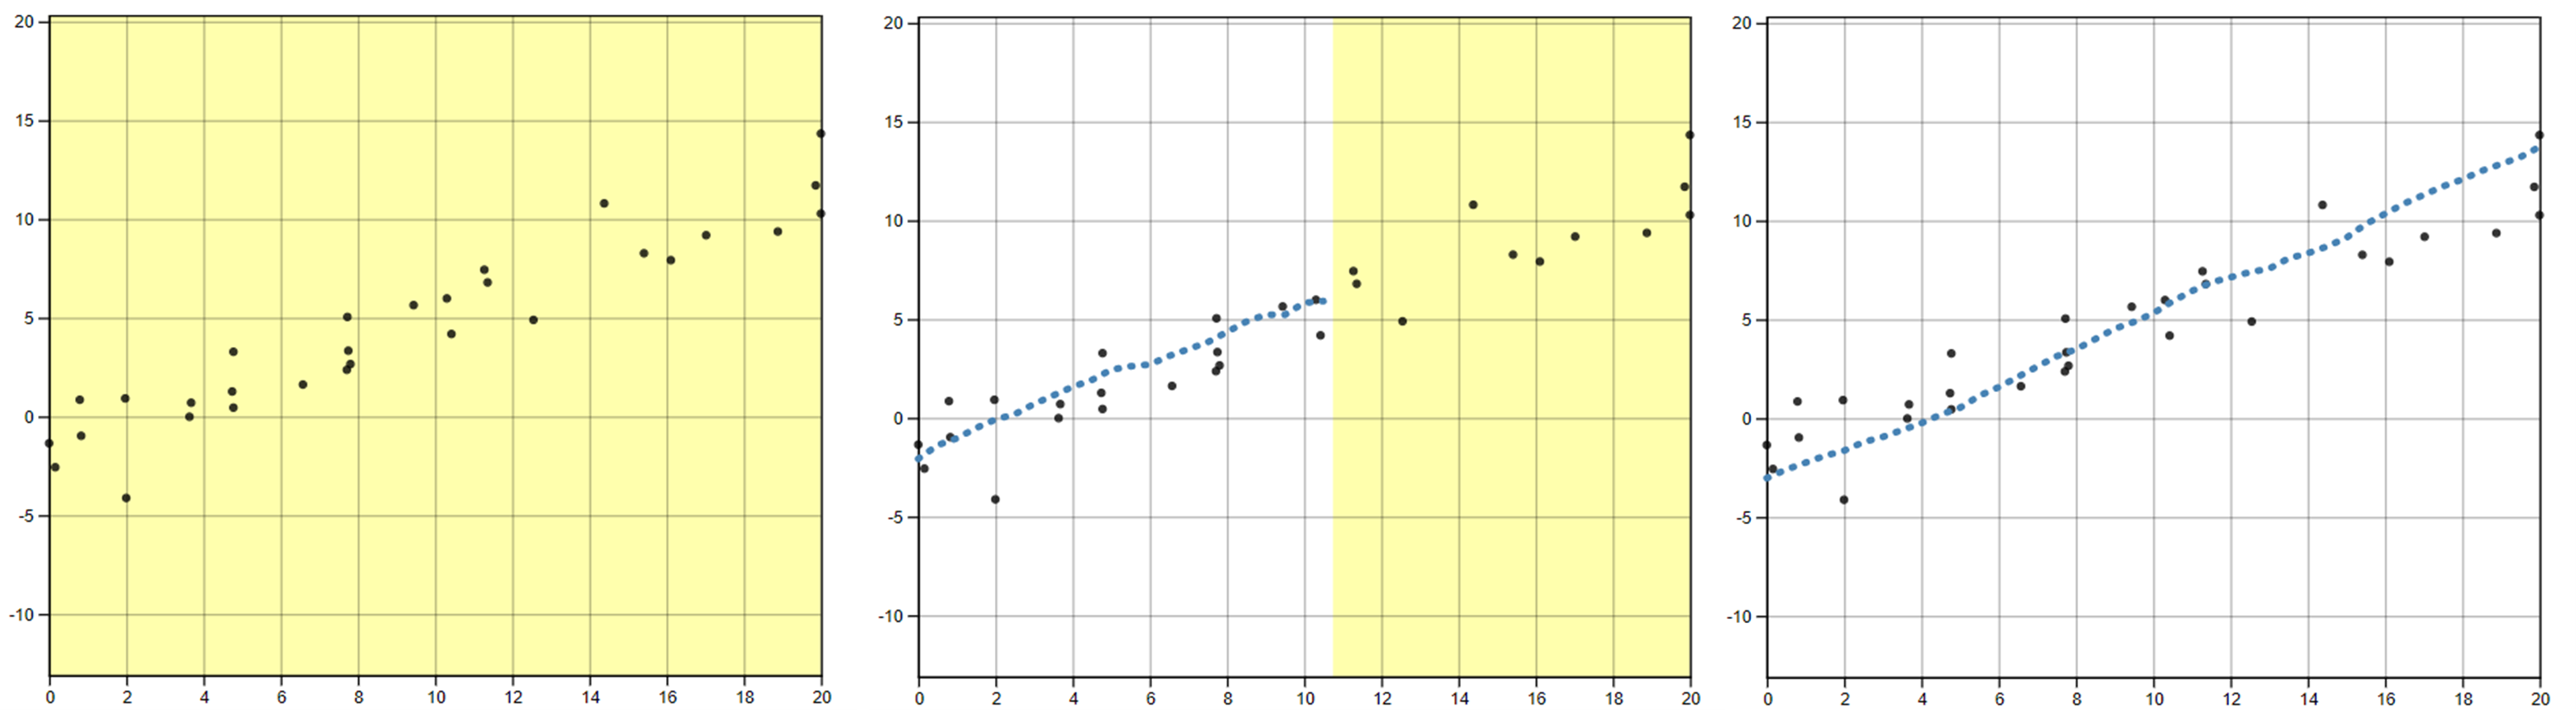
\includegraphics[width=1\linewidth,]{images/ydi-stimuli} 

}

\caption{'You Draw It' task plot as shown to particpants during the study. The first frame (left) illustrates what particpants first see with the prompt “Use your mouse to fill in the trend in the yellow box region.” The second frame (middle), illustrates what the particpant sees while completing the task; the yellow region provides a visual cue for participants indicating where the participant still needs to complete a trend-line. The last frame (right) illustrates the participants finished trend-line before submission.}\label{fig:ydi-stimuli}
\end{figure}

\hypertarget{data-generation}{%
\subsection{Data Generation}\label{data-generation}}

All data processing was conducted in R statistical software. A total of
\(N = 30\) points \((x_i, y_i), i = 1,...N\) were generated for
\(x_i \in [x_{min}, x_{max}]\) where \(x\) and \(y\) have a linear
relationship. Data were simulated based on a linear model with additive
errors: \begin{align}
y_i & = \beta_0 + \beta_1 x_i + e_i \\
\text{with } e_i & \sim N(0, \sigma^2). \nonumber
\end{align}

Model equation parameters, \(\beta_0\) and \(\beta_1\), were selected to
reflect the four data sets (F, N, S, and V) used in
\citet{mosteller1981eye} (\cref{tab:eyefitting-parameters}). Parameter
choices F, N, and S simulated data across a domain of 0 to 20. Parameter
choice F produces a trend with a positive slope and a large variance
while N has a negative slope and a large variance. In comparison, S
shows a trend with a positive slope with a small variance and V yields a
steep positive slope with a small variance over the domain of 4 to 16.
\cref{fig:eyefitting-simplot} illustrates an example of simulated data
for all four parameter choices intended to reflect the trends in
\citet{mosteller1981eye}. Aesthetic design choices were made consistent
across each of the interactive `You Draw It' task plots. The y-axis
range extended 10\% beyond (above and below) the range of the simulated
data points to allow for users to draw outside the simulated data set
range.

\begin{table}

\caption{\label{tab:eyefitting-parameters}Designated model equation parameters for simulated data.}
\centering
\begin{tabular}[t]{cccc}
\toprule
Parameter Choice & $y_{\bar{x}}$ & $\beta_1$ & $\sigma$\\
\midrule
S & 3.88 & 0.66 & 1.30\\
F & 3.90 & 0.66 & 1.98\\
V & 3.89 & 1.98 & 1.50\\
N & 4.11 & -0.70 & 2.50\\
\bottomrule
\end{tabular}
\end{table}

\begin{figure}[tbp]

{\centering 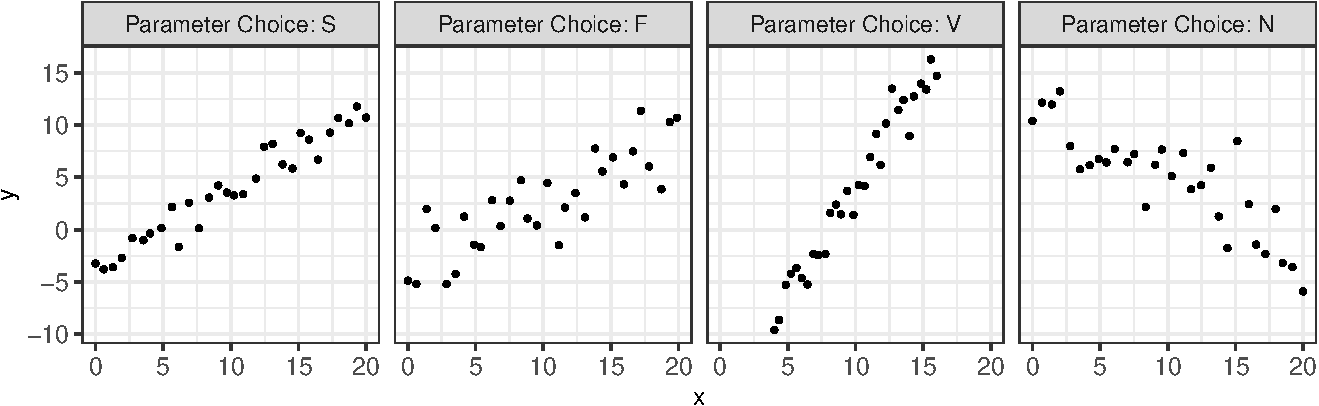
\includegraphics[width=1\linewidth,]{Eye-Fitting-Straight-Lines-in-the-Modern-Era_files/figure-latex/eyefitting-simplot-1} 

}

\caption{Example of simulated data points displayed in a scatter-plot illustrating the trends associated with the four selected parameter choices.}\label{fig:eyefitting-simplot}
\end{figure}

\hypertarget{study-design}{%
\subsection{Study Design}\label{study-design}}

This experiment was conducted as part of a larger study; for simplicity,
we focus on the study design and methods related to the current study.
Each scatter-plot was the graphical representation of a data set that
was generated randomly, independently for each participant at the start
of the experiment. Participants in the study are shown two `You Draw It'
practice plots in order to train participants in the skills associated
with executing the task. During the practice session, participants are
provided with instruction prompts accompanied by a .gif and a practice
plot. Instructions guide participants to start at the edge of the yellow
box, to make sure the yellow region is moving along with their mouse as
they draw, and that they can draw over their already drawn line.
Practice plots are then followed by four `You Draw It' task plots
associated with the current study. The order of the task plots was
randomly assigned for each individual in a completely randomized design.

\hypertarget{results}{%
\section{Results}\label{results}}

\hypertarget{fitted-regression-lines}{%
\subsection{Fitted Regression Lines}\label{fitted-regression-lines}}

We compare the participant drawn line to two regression lines determined
by ordinary least squares regression and regression based on the
principal axis (i.e.~Deming Regression). \cref{fig:ols-vs-pca-example}
illustrates the difference between an OLS regression line which
minimizes the vertical distance of points from the line and a regression
line based on the principal axis which minimizes the Euclidean distance
of points (orthogonal) from the line.

Due to the randomness in the data generation process, the actual slope
of the linear regression line fit through the simulated points could
differ from the predetermined slope. Therefore, we fit an ordinary least
squares (OLS) regression to each scatter-plot to obtain estimated
parameters \(\hat\beta_{0,OLS}\) and \(\hat\beta_{1,OLS}\). Fitted
values, \(\hat y_{k,OLS}\), are then obtained every 0.25 increments
across the domain from the OLS regression equation,
\(\hat y_{k,OLS} = \hat\beta_{0,OLS} + \hat\beta_{1,OLS} x_k\)., for
\(k = 1, ..., 4 x_{max} +1\). The regression equation based on the
principal axis was determined by using the \texttt{princomp} function in
the stats package in base R to obtain the rotation of the coordinate
axes from the first principal component (direction which captures the
most variance). The estimated slope, \(\hat\beta_{1,PCA}\), is
determined by the ratio of the axis rotation in y and axis rotation in x
of the first principal component with the y-intercept,
\(\hat\beta_{0,PCA}\) calculated by the point-slope equation of a line
using the mean of of the simulated points, \((\bar x_i, \bar y_i)\).
Fitted values, \(\hat y_{k,PCA}\), are then obtained every 0.25
increment across the domain from the PCA regression equation,
\(\hat y_{k,PCA} = \hat\beta_{0,PCA} + \hat\beta_{1,PCA} x_k\).

\begin{figure}[tbp]

{\centering 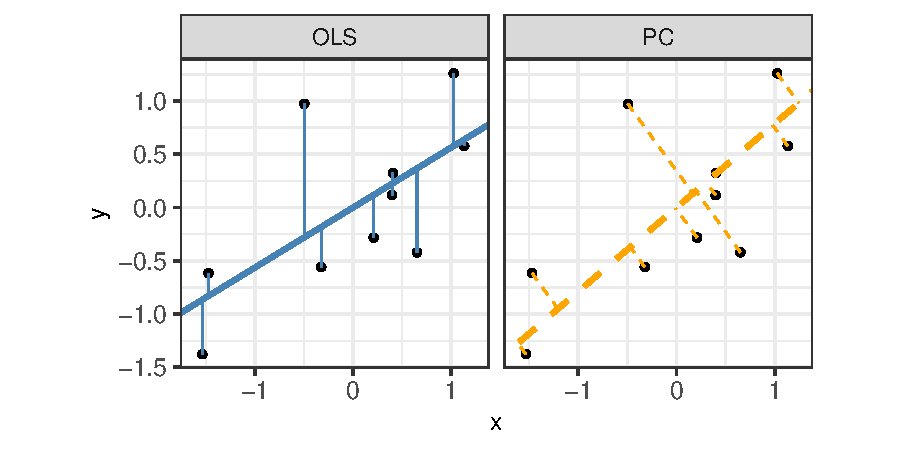
\includegraphics[width=0.8\linewidth,]{Eye-Fitting-Straight-Lines-in-the-Modern-Era_files/figure-latex/ols-vs-pca-example-1} 

}

\caption{ Comparison between an OLS regression line which minimizes the vertical distance of points from the line and a regression line based on the principal axis which minimizes the Euclidean distance of points (orthogonal) from the line.}\label{fig:ols-vs-pca-example}
\end{figure}

\hypertarget{residual-trends}{%
\subsection{Residual Trends}\label{residual-trends}}

For each participant, the final data set used for analysis contains
\(x_{ijk}, y_{ijk,drawn}, \hat y_{ijk,OLS}\), and \(\hat y_{ijk,PCA}\)
for parameter choice \(i = 1,2,3,4\), j = \(1,...N_{participant}\), and
\(x_{ijk}\) value \(k = 1, ...,4 x_{max} + 1\). Using both a linear
mixed model and a generalized additive mixed model, comparisons of
vertical residuals in relation to the OLS fitted values
(\(e_{ijk,OLS} = y_{ijk,drawn} - \hat y_{ijk,OLS}\)) and PCA fitted
values (\(e_{ijk,PCA} = y_{ijk,drawn} - \hat y_{ijk,PCA}\)) were made
across the domain. \cref{fig:eyefitting-example-plot} displays an
example of all three fitted trend lines for parameter choice F. Data
used in the analyses are available to be downloaded from GitHub
\href{https://github.com/earobinson95/Eye-Fitting-Straight-Lines-in-the-Modern-Era/raw/main/data/youdrawit-eyefitting-model-data.csv}{here}.

\begin{figure}[tbp]

{\centering 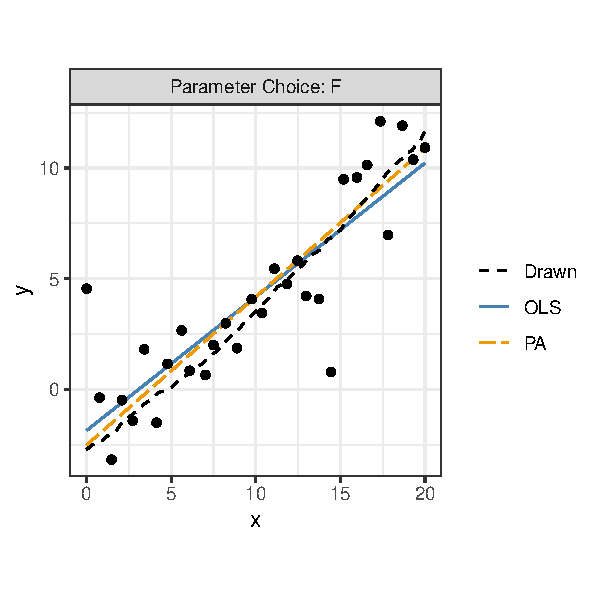
\includegraphics[width=0.5\linewidth,]{Eye-Fitting-Straight-Lines-in-the-Modern-Era_files/figure-latex/eyefitting-example-plot-1} 

}

\caption{Illustrates the data associated with and collected for one 'You Draw It' task plot. Trend-lines include the participant drawn line (dashed black), the OLS regression line (solid steelblue) and the PCA regression line based on the principal axis (solid orange).}\label{fig:eyefitting-example-plot}
\end{figure}

\hypertarget{linear-trend-constraint}{%
\subsubsection{Linear Trend Constraint}\label{linear-trend-constraint}}

Using the \texttt{lmer} function in the lme4 package \citep{lme4}, a
linear mixed model (LMM) is fit separately to the OLS residuals and PCA
residuals, constraining the fit to a linear trend. Parameter choice,
\(x\), and the interaction between \(x\) and parameter choice were
treated as fixed effects with a random participant effect accounting for
variation due to participant. The LMM equation for each fit (OLS and
PCA) is given by: \begin{equation}
y_{ijk,drawn} - \hat y_{ijk,fit} = e_{ijk,fit} = \left[\gamma_0 + \alpha_i\right] + \left[\gamma_{1} x_{ijk} + \gamma_{2i} x_{ijk}\right] + p_{j} + \epsilon_{ijk}
\end{equation} \noindent where

\begin{itemize}
\tightlist
\item
  \(y_{ijk,drawn}\) is the drawn y-value for the \(i^{th}\) parameter
  choice, \(j^{th}\) participant, and \(k^{th}\) increment of x-value
\item
  \(\hat y_{ijk,fit}\) is the fitted y-value for the \(i^{th}\)
  parameter choice, \(j^{th}\) participant, and \(k^{th}\) increment of
  x-value corresponding to either the OLS or PCA fit
\item
  \(e_{ijk,fit}\) is the residual between the drawn and fitted y-values
  for the \(i^{th}\) parameter choice, \(j^{th}\) participant, and
  \(k^{th}\) increment of x-value corresponding to either the OLS or PCA
  fit
\item
  \(\gamma_0\) is the overall intercept
\item
  \(\alpha_i\) is the effect of the \(i^{th}\) parameter choice (F, S,
  V, N) on the intercept
\item
  \(\gamma_1\) is the overall slope for \(x\)
\item
  \(\gamma_{2i}\) is the effect of the parameter choice on the slope
\item
  \(x_{ijk}\) is the x-value for the \(i^{th}\) parameter choice,
  \(j^{th}\) participant, and \(k^{th}\) increment
\item
  \(p_{j} \sim N(0, \sigma^2_{participant})\) is the random error due to
  the \(j^{th}\) participant's characteristics
\item
  \(\epsilon_{ijk} \sim N(0, \sigma^2)\) is the residual error.
\end{itemize}

Constraining the residual trend to a linear fit,
\cref{fig:eyefitting-lmer-residualplots} shows the estimated trend line
of the residuals between the participant drawn points and fitted values
for both the OLS regression line and PCA regression line. Estimated
residual trend lines are overlaid on the observed individual participant
residuals. Results indicate the estimated trends of PCA residuals
(orange) appear to align closer to the \(y=0\) horizontal (dashed) line
than the OLS residuals (blue). In particular, this trend is more
prominent in parameter choices with large variances (F and N). These
results are consistent to those found in \citet{mosteller1981eye}
indicating participants fit a trend-line closer to the estimated
regression line with the slope of based on the first principal axis than
the estimated OLS regression line thus, providing support for ``ensemble
perception''.

\begin{figure}[tbp]

{\centering 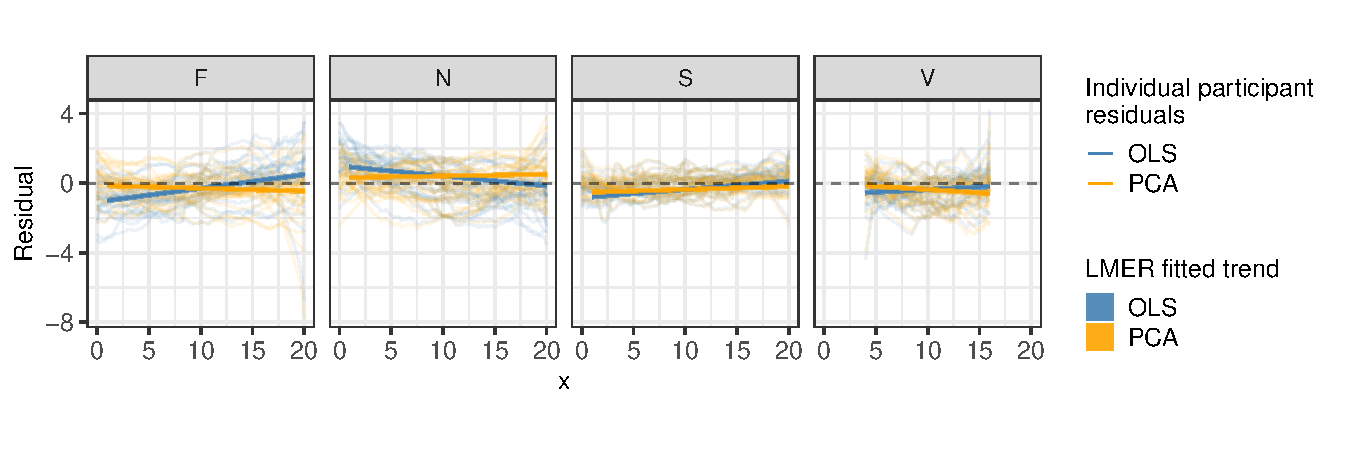
\includegraphics[width=1\linewidth,]{Eye-Fitting-Straight-Lines-in-the-Modern-Era_files/figure-latex/eyefitting-lmer-residualplots-1} 

}

\caption{Eye Fitting Straight Lines in the Modern Era LMM results}\label{fig:eyefitting-lmer-residualplots}
\end{figure}

\hypertarget{smoothing-spline-trend}{%
\subsubsection{Smoothing Spline Trend}\label{smoothing-spline-trend}}

Eliminating the linear trend constraint, the \texttt{bam} function in
the mgcv package \citep{mgcv1, mgcv2, mgcv3, mgcv4, mgcv5} is used to
fit a generalized additive mixed model (GAMM) separately to the OLS
residuals and PCA residuals to allow for estimation of smoothing
splines. Parameter choice was treated as a fixed effect with no
estimated intercept and a separate smoothing spline for \(x\) was
estimated for each parameter choice. A random participant effect
accounting for variation due to participant and a random spline for each
participant accounted for variation in spline for each participant. The
GAMM equation for each fit (OLS and PCA) residuals is given by:
\begin{equation}
y_{ijk, drawn} - \hat y_{ijk, fit} = e_{ijk,fit} = \alpha_i + s_{i}(x_{ijk}) + p_{j} + s_{j}(x_{ijk})
\end{equation} \noindent where

\begin{itemize}
\tightlist
\item
  \(y_{ijk,drawn}\) is the drawn y-value for the \(i^{th}\) parameter
  choice, \(j^{th}\) participant, and \(k^{th}\) increment of x-value
\item
  \(\hat y_{ijk,fit}\) is the fitted y-value for the \(i^{th}\)
  parameter choice, \(j^{th}\) participant, and \(k^{th}\) increment of
  x-value corresponding to either the OLS or PCA fit
\item
  \(e_{ijk,fit}\) is the residual between the drawn and fitted y-values
  for the \(i^{th}\) parameter choice, \(j^{th}\) participant, and
  \(k^{th}\) increment of x-value corresponding to either the OLS or PCA
  fit
\item
  \(\alpha_i\) is the intercept for the parameter choice \(i\)
\item
  \(s_{i}\) is the smoothing spline for the \(i^{th}\) parameter choice
\item
  \(x_{ijk}\) is the x-value for the \(i^{th}\) parameter choice,
  \(j^{th}\) participant, and \(k^{th}\) increment
\item
  \(p_{j} \sim N(0, \sigma^2_{participant})\) is the error due to
  participant variation
\item
  \(s_{j}\) is the random smoothing spline for each participant.
\end{itemize}

Allowing for flexibility in the residual trend,
\cref{fig:eyefitting-gamm-residualplots} shows the estimated trend line
of the residuals between the participant drawn points and fitted values
for both the OLS regression line and PCA regression line. Estimated
residual trends are overlaid on the observed individual participant
residuals. The results of the GAMM align with those shown in
\cref{fig:eyefitting-lmer-residualplots} providing support that for
scatter-plots with more noise (F and N), estimated trends of PCA
residuals (orange) appear to align closer to the \(y=0\) horizontal
(dashed) line than the OLS residuals (blue). By fitting smoothing
splines, we can determine whether participants naturally fit a straight
trend-line to the set of points or whether they deviate throughout the
domain. In particular, in scatter-plots with smaller variance (S and V),
we can see that participants began at approximately the correct starting
point then deviated away from the fitted regression lines and correcting
for their fit toward the end of their trend-line. In scatter-plots with
larger variance (F and N), participants estimated their starting value
in the extreme direction of the OLS regression line based on the
increasing or decreasing trend but more accurately represented the
starting value of the PCA regression line. As participants continued
their trend-line, they crossed through the OLS regression line
indicating they estimated the slope in the extreme direction. These
results provide further insight into the curvature humans perceive in a
set of points.

\begin{figure}[tbp]

{\centering 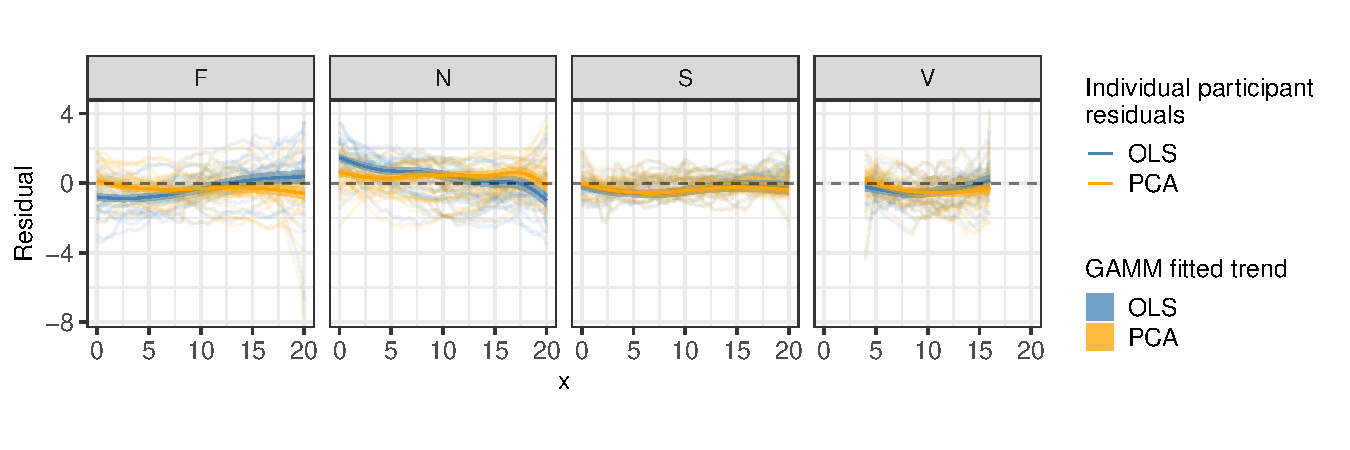
\includegraphics[width=1\linewidth,]{Eye-Fitting-Straight-Lines-in-the-Modern-Era_files/figure-latex/eyefitting-gamm-residualplots-1} 

}

\caption{Eye Fitting Straight Lines in the Modern Era GAMM results}\label{fig:eyefitting-gamm-residualplots}
\end{figure}

\hypertarget{discussion-and-conclusion}{%
\section{Discussion and Conclusion}\label{discussion-and-conclusion}}

The intent of research was to adapt `You Draw It' from the New York
Times feature as a tool and method for testing graphics The study
conducted by \citet{mosteller1981eye} was replicated using the `You Draw
It' method providing support for the validity of the tool. Our results
indicated that when shown points following a linear trend, participants
tended to fit a line closer to a regression based on the principal axis
over the ordinary least squares regression line. This trend was most
prominent when shown data simulated with larger variances. These results
indicate that humans perform ``ensemble perception'' in a statistical
graphic setting as participants minimized the distance from the their
regression line over both the \(x\) and \(y\) axis simultaneously. In
addition, we allowed participants to draw trend lines that deviated from
a straight line providing insight into the curvature the human eye
perceives in a set of points.

\hypertarget{future-work}{%
\section{Future Work}\label{future-work}}

This study provided a basis for the use of `You Draw It' as a tool for
testing graphics as well as provided support for ``ensemble perception''
in statistical graphics. Further investigation is necessary to implement
the method in non-linear settings and with real data. This tool could
also be used to evaluate human ability to extrapolate data from trends.
In the future, an R package designed for easy implementation of `You
Draw It' task plots will help make this tool accessible to other
researchers.

\bibliographystyle{agsm}
\bibliography{bibliography.bib}

\end{document}
